El aseguramiento de la calidad (QA) en sistemas descentralizados representa un cambio de paradigma respecto a la ingeniería de software tradicional, principalmente debido a la inmutabilidad de la lógica de negocio y la ejecución distribuida de procesos. A diferencia de los sistemas centralizados, donde el mantenimiento correctivo permite parches post-implantación, la naturaleza de la blockchain exige que el testing sea exhaustivo, preventivo y multidimensional antes de cualquier despliegue en la red principal (Mainnet).

\subsection*{A. Verificación Formal y Security Testing en Contratos Inteligentes}
La seguridad se constituye como el eje crítico en el ciclo de vida del testing para blockchain. Según las investigaciones de Tolmach et al., la lógica de negocio en entornos descentralizados es vulnerable a vectores de ataque como la reentrada y desbordamientos aritméticos, los cuales, en un sistema de notas, podrían permitir la alteración no autorizada de promedios \cite{tolmach2021survey}. El análisis estático y la verificación formal surgen como métodos para asegurar que el contrato se comporte según lo especificado en todos los estados posibles. Sin embargo, la literatura señala que estos métodos presentan una alta barrera de entrada debido a su complejidad técnica y el costo computacional asociado \cite{tolmach2021survey}.

\subsection*{B. Infraestructura de Testing en el Ecosistema Polkadot y Substrate}

Polkadot utiliza el framework Substrate, el cual implementa una arquitectura basada en un runtime compilado a WebAssembly (WASM). Según la documentación oficial de Parity Technologies, el testing en este entorno se divide en tres capas fundamentales: pruebas unitarias sobre paletas individuales, pruebas de integración usando el entorno MockRuntime y pruebas de regresión para asegurar la compatibilidad en las actualizaciones sin bifurcaciones (forkless upgrades) \cite{parity2024substrate}. Esta capacidad de actualización, única de Substrate, requiere una suite de pruebas que valide que la migración del estado de las notas académicas sea atómica y no corrompa la integridad de los datos históricos preexistentes \cite{parity2024substrate}.

\begin{figure}[H]
    \centering
    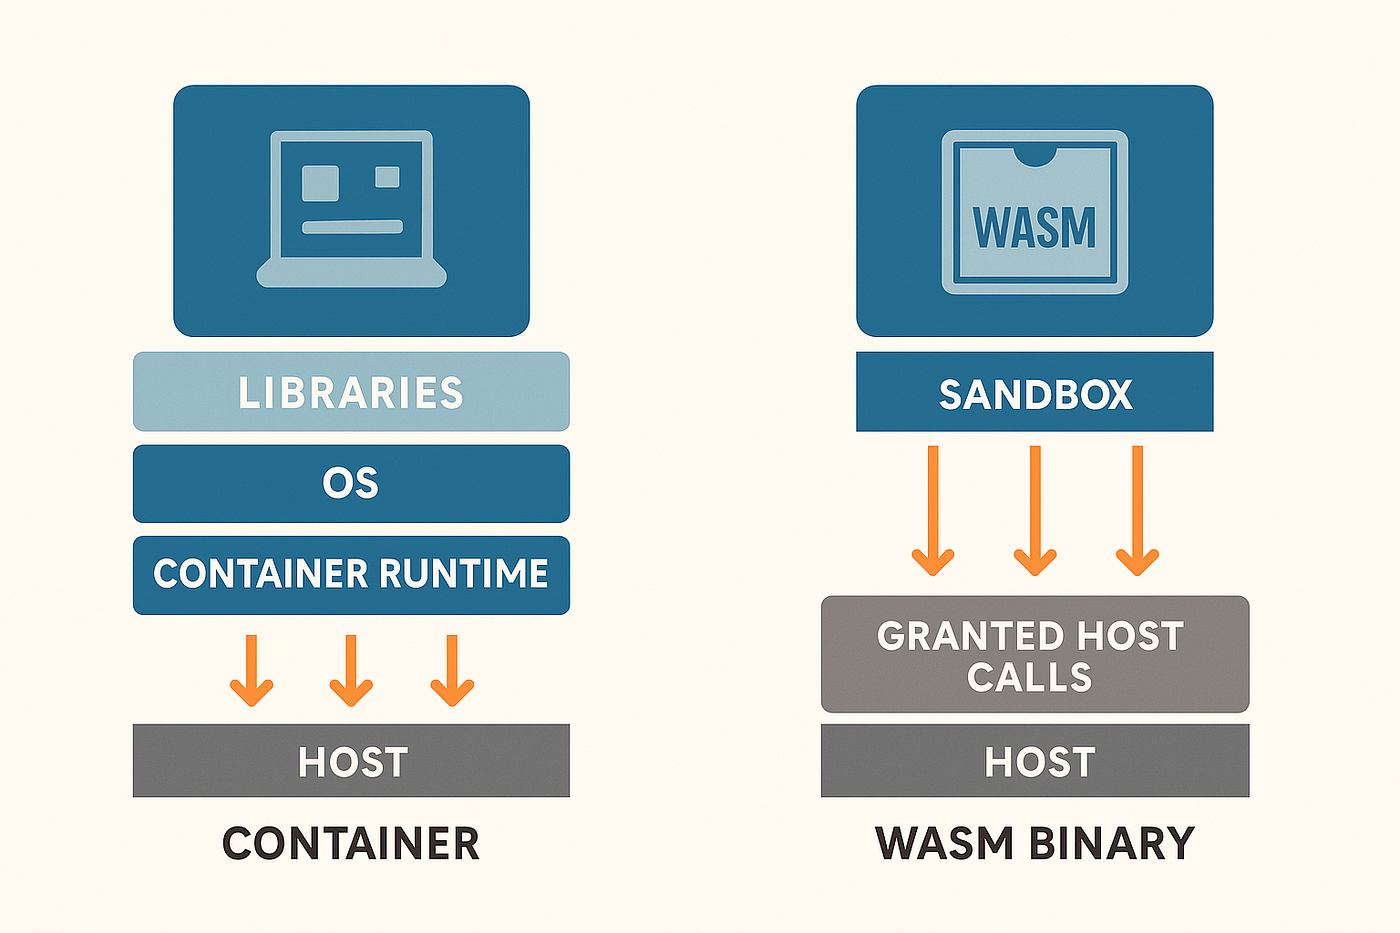
\includegraphics[width=\columnwidth]{media/estado_arte/2026-04-24-23-16-59.png}
    \captionof{figure}{Diferencia con WASM}
    \label{fig:fig1}
\end{figure}


\subsection*{C. Interoperabilidad y Testing de Mensajería Cross-Chain (XCM)}

Un sistema de notas moderno sobre Polkadot no opera de forma aislada, sino que interactúa con otras parachains mediante el formato de mensajes XCM (Cross-Consensus Messaging). Investigaciones recientes presentadas en IEEE destacan que el testing de interoperabilidad es crítico para evitar fallos en la comunicación asíncrona entre cadenas \cite{stefanko2023paraspell}. Herramientas como ParaSpell han demostrado que la validación de mensajes XCM en entornos de prueba (testnets) reduce significativamente el tiempo de ejecución de transacciones y asegura que las credenciales académicas transferidas entre diferentes redes mantengan su validez criptográfica \cite{stefanko2023paraspell}.

\begin{figure}[H]
    \centering
    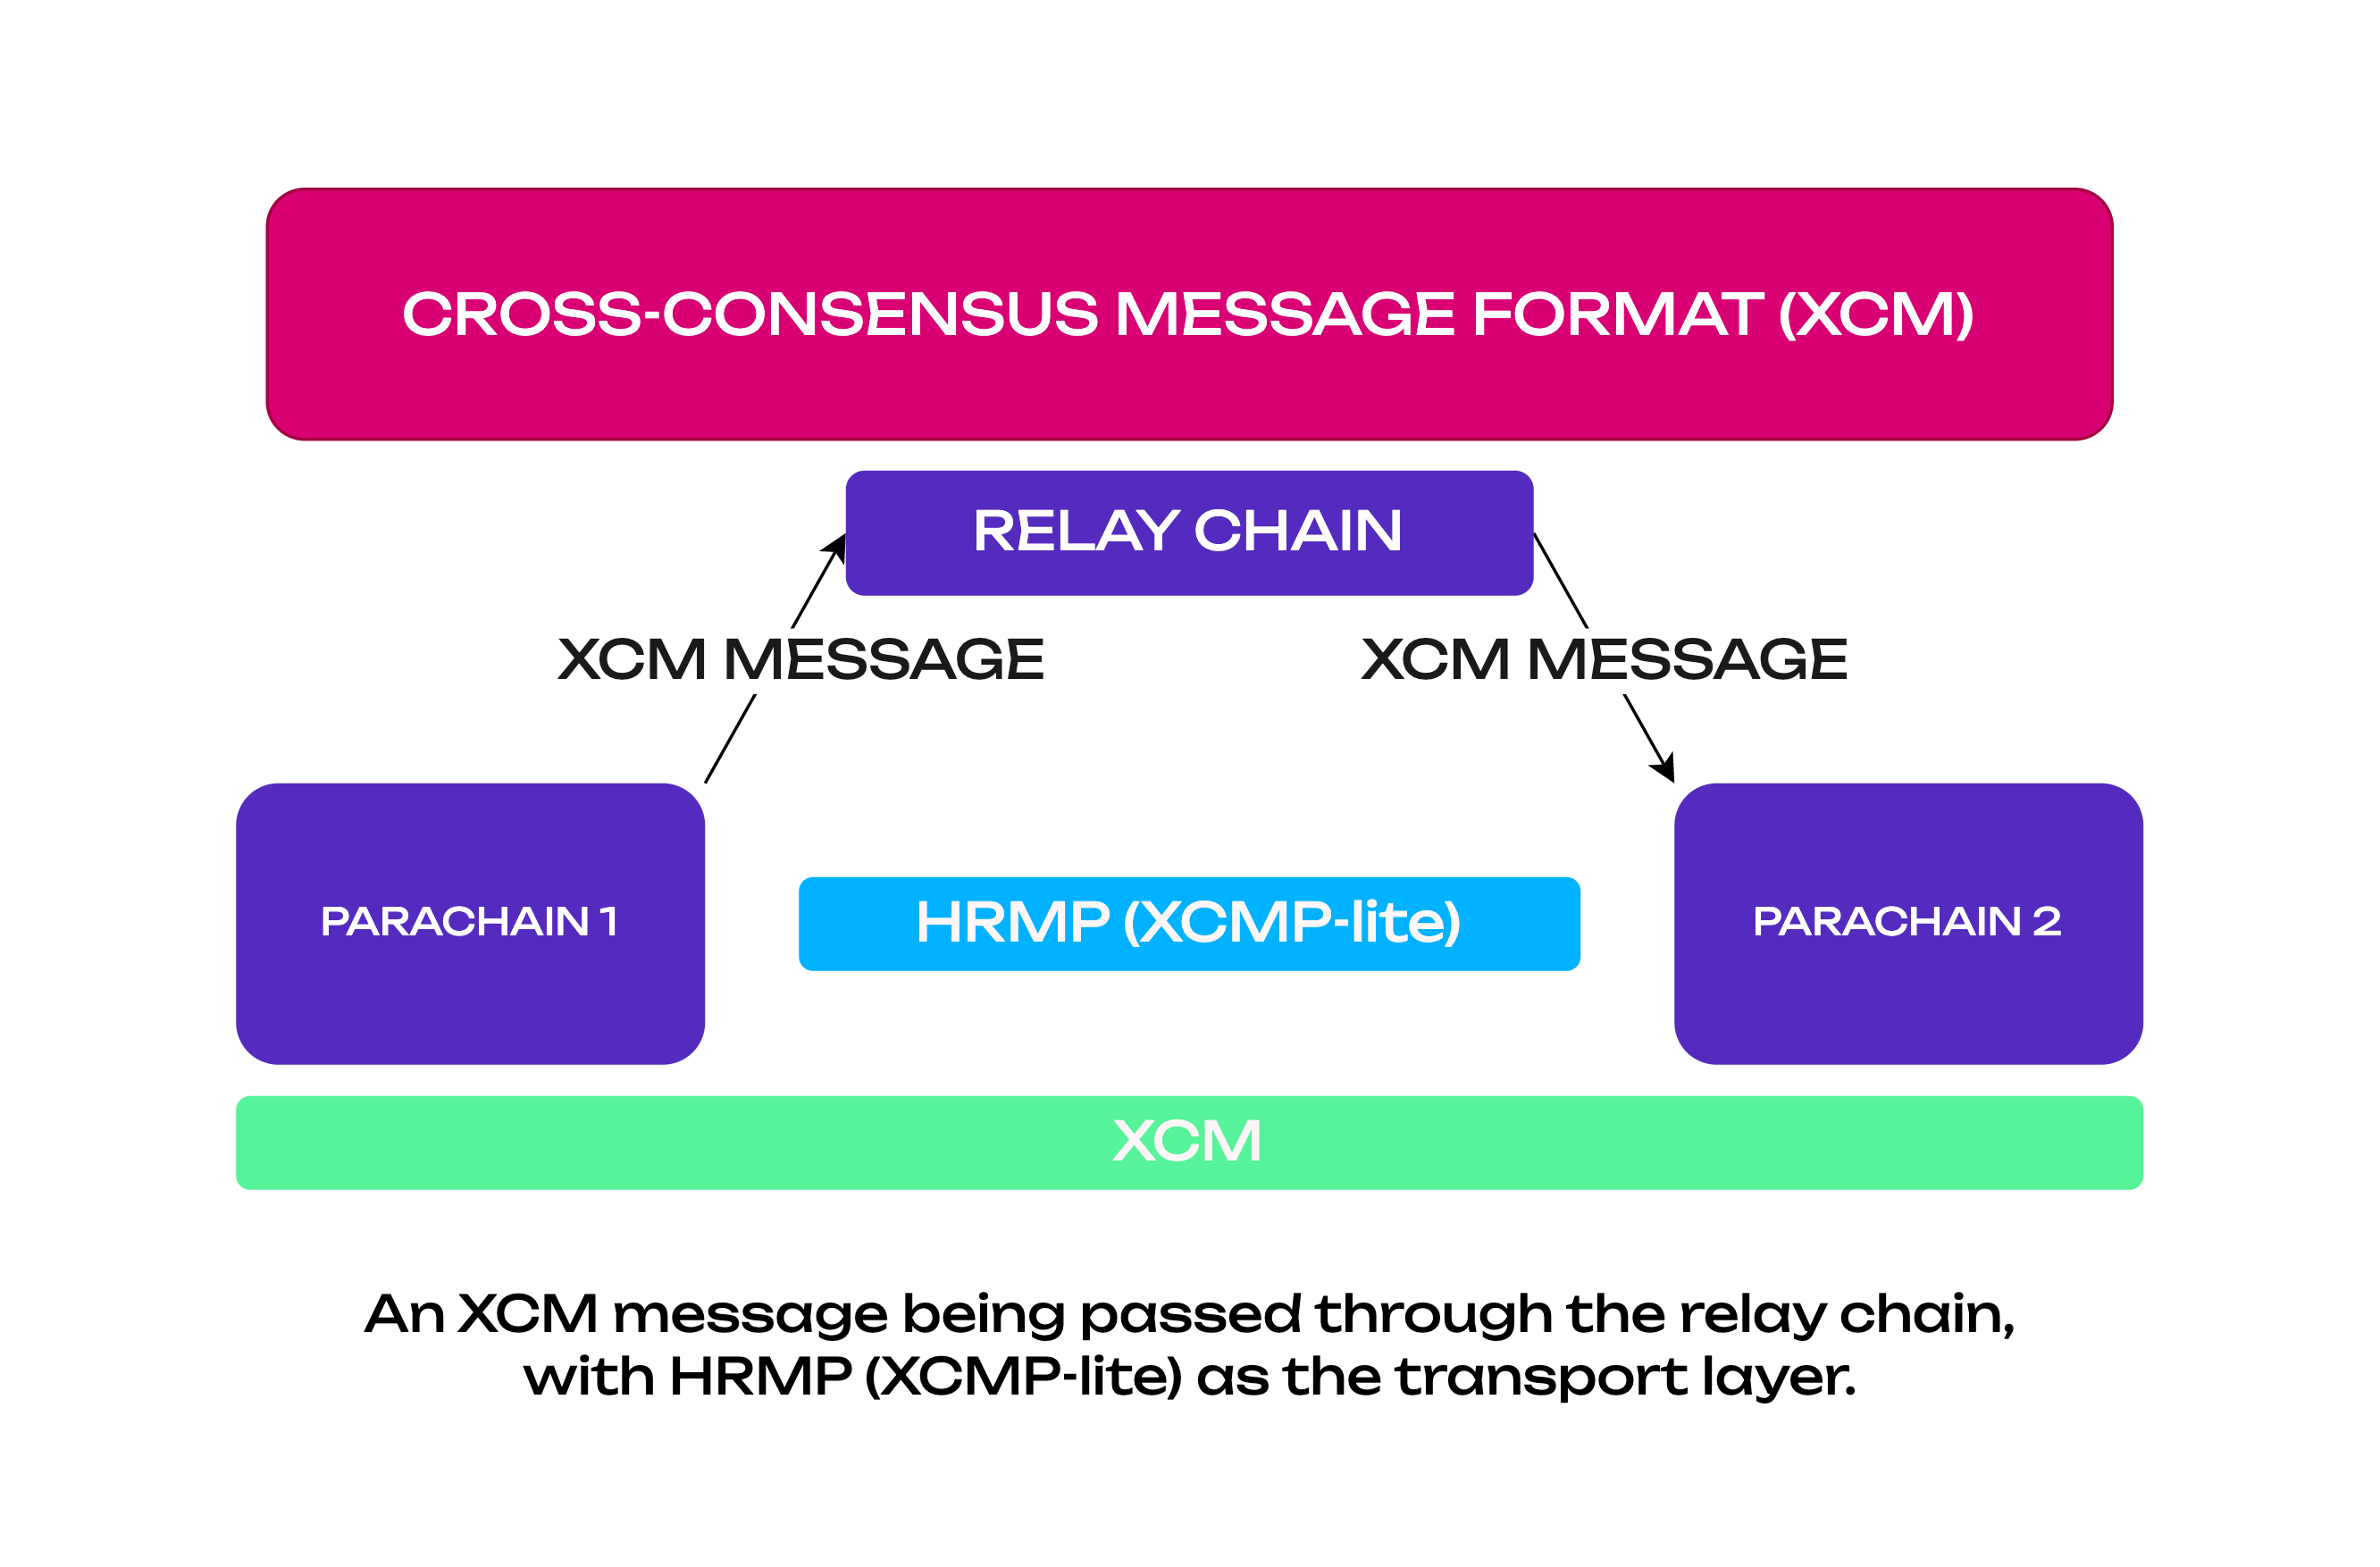
\includegraphics[width=\columnwidth]{media/estado_arte/2026-04-24-23-20-17.png}
    \captionof{figure}{Horizontal Relay-routed Message Passing (HRMP)}
    \label{fig:HRMP}
\end{figure}

\subsection*{D. Mutation Testing y Evaluación de Suites de Pruebas}

Para elevar el estándar de calidad, se ha propuesto el uso de Mutation Testing (Pruebas de Mutación). Según Gao et al., esta técnica consiste en inyectar fallos artificiales (mutantes) en el código del contrato para verificar si la suite de pruebas existente es capaz de detectarlos \cite{gao2022blockchain}. En entornos de Smart Contracts, esto es vital para identificar "pruebas débiles" que podrían dejar pasar vulnerabilidades lógicas. El estudio de herramientas como SuMo para Solidity y su extrapolación a contratos en Rust/ink! sugiere que la cobertura de código tradicional no es suficiente, siendo necesaria una métrica de "puntuación de mutación" para garantizar la robustez del sistema \cite{bernardi2021sumo}.

\subsection*{E. Testing de No-determinismo en Off-chain Workers}

Una de las funcionalidades avanzadas de Substrate son los Off-chain Workers (OCW), los cuales permiten realizar tareas pesadas (como llamados a APIs universitarias externas) fuera de la cadena. La documentación de Polkadot advierte que el testing de OCWs presenta desafíos únicos debido al no-determinismo inherente de las peticiones HTTP \cite{polkadotwiki2024ocw}. El proceso de QA debe incluir mocking de servicios externos y validación de firmas digitales para asegurar que los datos que ingresan a la blockchain (las notas externas) sean verificables y no comprometan el consenso de la red \cite{polkadotwiki2024ocw}.

\begin{figure}[H]
    \centering
    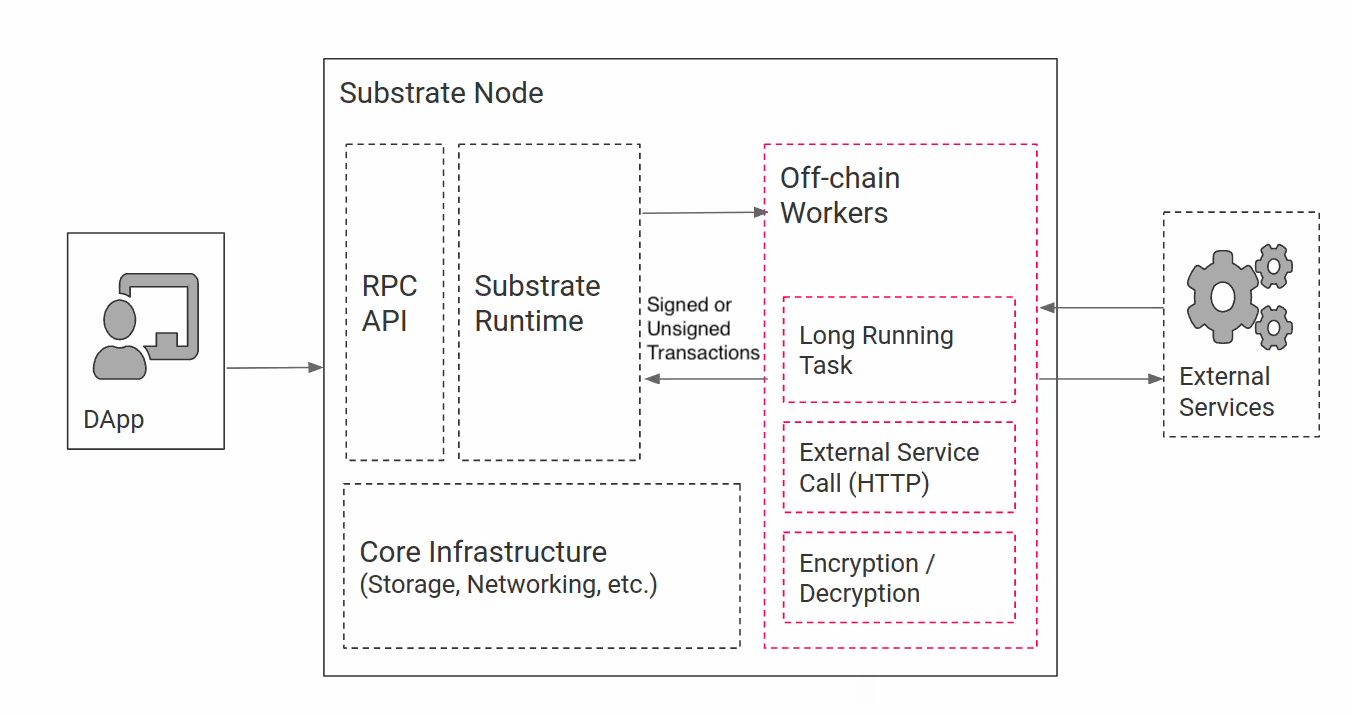
\includegraphics[width=\columnwidth]{media/estado_arte/2026-04-24-23-24-21.png}
    \captionof{figure}{Offchain Workers}
    \label{fig:OCW}
\end{figure}
